\chapter{Experimentación}\label{ch:Experimentación}

Este capítulo tiene como objetivo mostrar el correcto funcionamiento las funciones documentadas en el Capítulo \ref{ch:Impl}. Para ello las aplicaremos sobre conjuntos de datos correspondientes a casos de aplicación reales, así como a conjuntos artificiales.

Cabe destacar que los parámetros dados como argumento a las funciones son los especificados por defecto en el Capítulo \ref{ch:Impl} a no ser que se especifique lo contrario, es decir, no se han optimizado para los datos concretos a los que se aplican en cada ocasión. La optimización de parámetros queda a cargo del usuario, que deberá realizar un estudio sobre los mismos para adaptarlos al problema concreto que intenta resolver.

\section{Conjuntos de datos considerados} \label{datasets}

Tal y como ya se ha mencionado, tomaremos conjuntos de datos reales y artificiales para poner a prueba los 5 métodos implementados. Teniendo en cuenta dicha distinción, a continuación se detallan los pormenores de cada uno de ellos.

\subsection{Conjuntos de datos reales}

Consideraremos 4 conjuntos de datos correspondientes a casos reales de aplicación de técnicas de \acf{AA}:

\begin{itemize}
	
	\item \textbf{Conjunto de datos \textit{Iris}}: el conjunto de datos Iris (\textit{Iris Dataset}) es uno de los más empleados en \acs{AA}. Famoso por ser objeto del primer intento de aplicación de métodos de clustering por el biólogo Ronald Fisher en 1936, quien intentaba obtener un método para clasificar flores de la especie Iris en sus tres subespecies: \textit{iris setosa}, \textit{iris virginica} e \textit{iris versicolor}. Compuesto por un total de 150 muestras de 3 clases distintas, caracterizadas cada una por 4 atributos en el dominio de los números reales positivos, a saber: altura del sépalo, anchura del sépalo, altura del pétalo y anchura del pétalo. Por facilidad de representación solo consideraremos las dos primeras características. La figura \ref{fig:figure27} muestra la distribución de las mismas.
	
	\item \textbf{Conjunto de datos \textit{Wine}}: el conjunto de datos Wine (\textit{Wine Dataset}) recoge 178 muestras de 3 clases de vinos distintas, caracterizadas cada una por 13 atributos en el dominio de los números reales positivos. Algunos de estos atributos son: contenido de alcohol, contenido de ácido málico, contenido de magnesio, etc.
	
	\item \textbf{Conjunto de datos \textit{Breast Cancer}}: el conjunto de datos Breast Cancer (\textit{Breast Cancer Dataset}) recoge 569 instancias asociadas cada una a una paciente que padecía o no de cáncer de mama (2 clases); cada muestra viene caracterizada por 30 atributos en el dominio de los números reales positivos. Algunos de los atributos son: edad de la paciente, tamaño del tumor, mama afectada, etc.
	
	\item \textbf{Conjunto de datos \textit{Glass}}: el conjunto de datos Glass (\textit{Glass Dataset}) recoge 214 muestras de 6 clases de cristal distintas, caracterizadas cada una por 10 atributos en multitud de dominios. Algunos de estos atributos son: indice reactivo, contenido en magnesio, contenido en aluminio, finalidad de uso, etc.
	
	\item \textbf{Conjunto de datos \textit{Digits}}: el conjunto de datos Digits (\textit{Digits Dataset}) recoge 1797 muestras de 10 clases de distintas, correspondientes a los dígitos manuscritos del 0 al 9. Cada muestra viene caracterizada por 64 atributos en el dominio de los enteros del 1 al 16.
	
\end{itemize}

La tabla \ref{tab:tabla7} muestra de manera resumida las características de estos 5 conjuntos de datos.

\begin{table}[h]
	\centering
	\setlength{\arrayrulewidth}{1mm}
	\setlength{\tabcolsep}{10pt}
	\renewcommand{\arraystretch}{0.75}
	
	\rowcolors{2}{gray!25}{white}
	\begin{tabular}{ >{\centering\arraybackslash}m{2.5cm}  >{\centering\arraybackslash}m{1.5cm}>{\centering\arraybackslash}m{1.5cm}>{\centering\arraybackslash}m{1.5cm}>{\centering\arraybackslash}m{1.5cm}}
		\hline
		\rowcolor{black}
		\multicolumn{5}{c}{\bf \color{white}{Conjuntos de datos reales}}\\
		\hline
		\rowcolor{gray!50}
		\textbf{Nombre} & \textbf{Muestras} & \textbf{Atributos} & \textbf{Clases} & \textbf{Dominio} \\
		Iris & $150$ & $4$ & $3$ & $\mathbb{R}^+$ \\
		Wine & $178$ & $13$ & $3$ & $\mathbb{R}^+$ \\
		Breast Cancer & $569$ & $30$ & $2$ & $\mathbb{R}^+$ \\
		Glass & $214$ & $10$ & $6$ & Varios \\
		Digits & $1797$ & $64$ & $10$ & $\{0-16\}$ \\
		\hline
		
	\end{tabular}
	\caption{Características de los conjuntos de datos reales considerados.}
	\label{tab:tabla7}
\end{table}

\begin{figure}[!h]
	\centering
	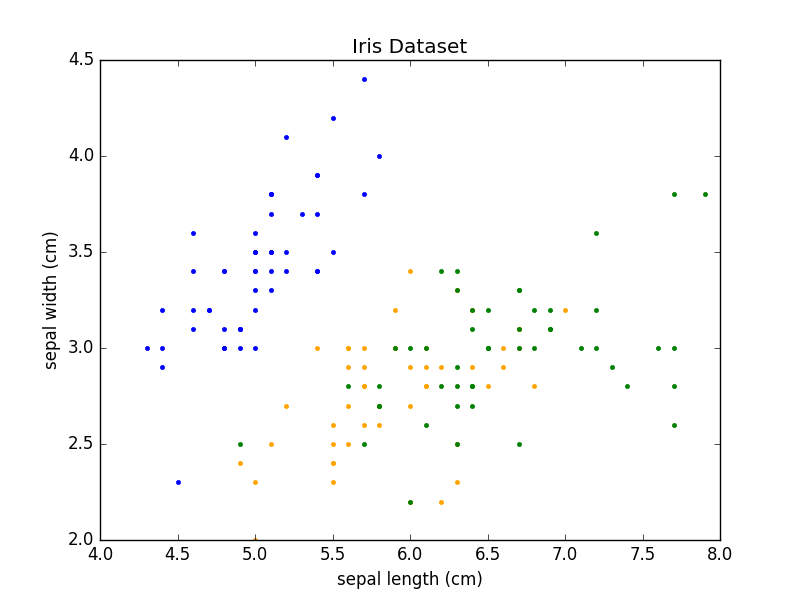
\includegraphics[scale=0.32]{imagenes/c6/IrisSet}
	\caption{Distribución de las dos primeras características de \textit{Iris Dataset}.}\label{fig:figure27}
\end{figure}

\subsection{Conjuntos de datos artificiales} \label{ArtifDataset}

En el caso de los conjuntos de datos artificiales el objetivo es generar clusters con una geometría concreta. Para ello sólo son necesarios dos atributos ($x$ e $y$) y un número de muestras arbitrario.

La Figura \ref{fig:figure22} muestra los 4 conjuntos de datos generados de manera artificial. Por simplicidad nos referiremos a cada uno de ellos por su identificador en inglés, que aparece en la anotación bajo cada imagen.

\begin{figure}[bth]
	\myfloatalign
	\subfloat[\textit{Rand Dataset}]
	{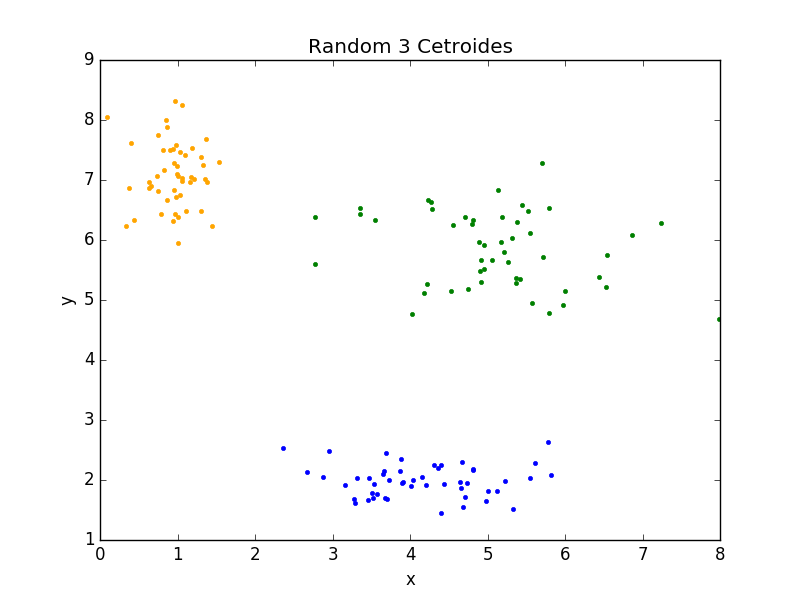
\includegraphics[width=.4\linewidth]{imagenes/c6/ArtifSets/RandSet}}
	\subfloat[\textit{Spirals Dataset}]
	{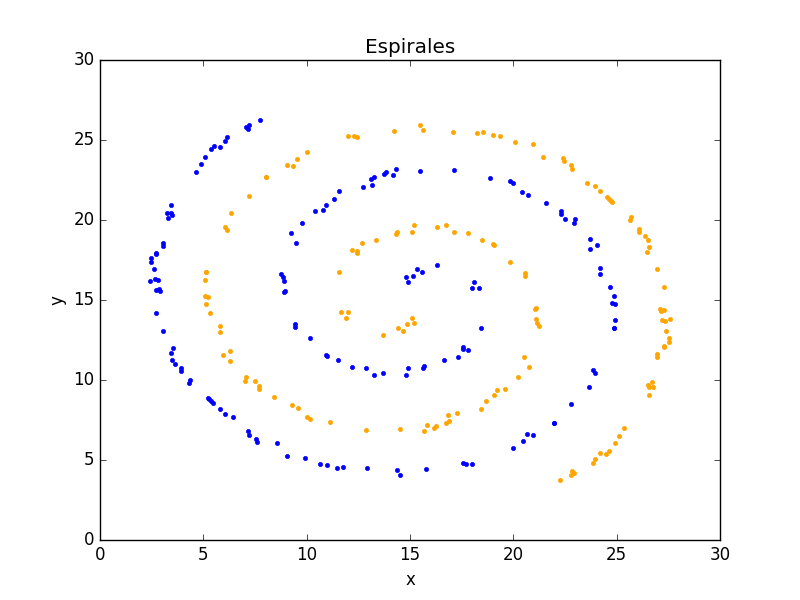
\includegraphics[width=.4\linewidth]{imagenes/c6/ArtifSets/SpiralSet}}\\
	\subfloat[\textit{Circles Dataset}]
	{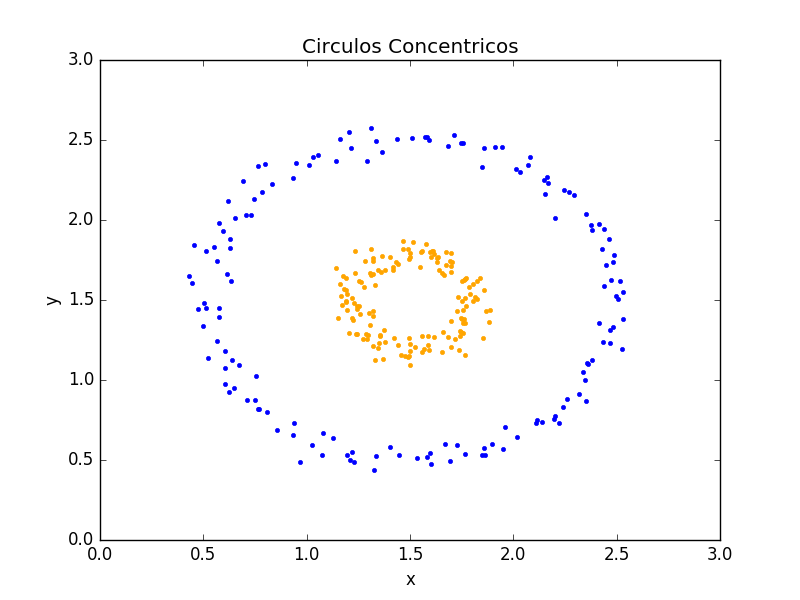
\includegraphics[width=.4\linewidth]{imagenes/c6/ArtifSets/Circles}}
	\subfloat[\textit{Moons Dataset}]
	{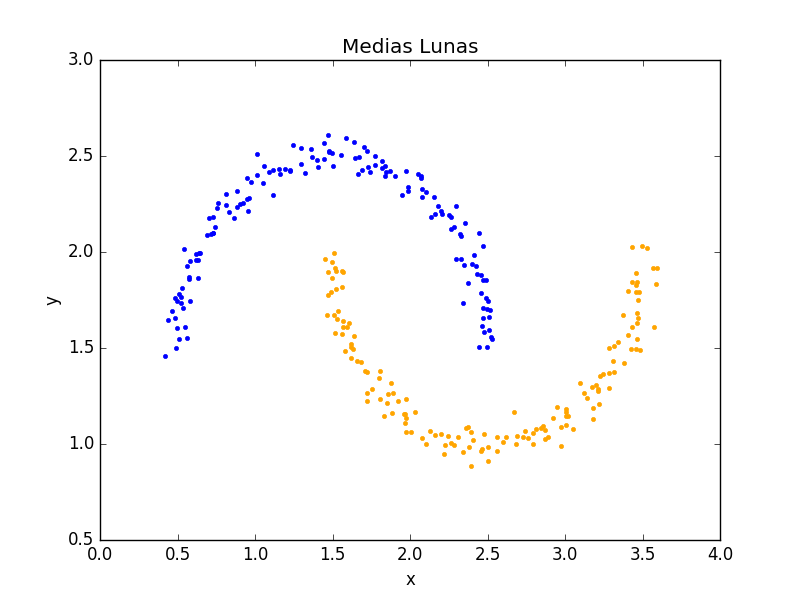
\includegraphics[width=.4\linewidth]{imagenes/c6/ArtifSets/MoonsSet}}
	\caption{Conjuntos de datos artificiales.}\label{fig:figure22}
\end{figure}

\section{Medida del error}

Tomamos la medida del error que Wagstaff et al. (2001) \cite{Wagstaff:2001b}, los autores de COP-K-medias, proponen en su trabajo para evaluar los resultados.

Dado que en la experimentación disponemos de las etiquetas verdaderas asociadas a cada uno de los conjuntos de datos, podemos hacer uso de las mismas en el post-procesado para evaluar los resultados que proporciona cada método.

Para calcular la exactitud de las predicciones resultado de cada método emplearemos \textit{Rand Index} \cite{Rand:1971}, que calcula el grado de similitud entre dos particiones dadas $P_1$ y $P_2$ del mismo conjunto de datos $X$.

Interpretamos cada partición como una colección de $n (n-1) / 2$ decisiones de emparejamiento, donde $n$ es el número de instancias en $X$. Para cada par de instancias $x_i$ y $x_j$ en $X$, $P_i$ las asigna al mismo cluster o a clusters diferentes. Tomamos $a$ como el número de emparejamientos donde $x_i$ está en el mismo cluster que $x_j$ en $P_1$ y $P_2$, y tomamos $b$ como el suceso contrario. Entonces, el grado de similitud entre $P_1$ y $P_2$ se calcula como:

\begin{equation}
Rand(P_1, P_2) = \frac{a + b}{n (n-1) / 2}
\label{eqn70}
\end{equation}

Ésta será la medida del error que emplearemos en todos los experimentos.

\section{Generación de las restricciones}

Para generar las restricciones haremos uso de la función propuesta para ello en la Sección \ref{genConst}. La cantidad de restricciones viene definida como un porcentaje aplicado sobre el cardinal del conjunto de datos. Dicho porcentaje se especificará en la sección correspondiente al análisis de cada algoritmo. No obstante, podemos obtener una representación gráfica de las restricciones haciendo uso de las funcionalidades de la biblioteca Matplotlib. La Figura \ref{fig:figure23} muestra las restricciones generadas sobre los conjuntos de datos \textit{Iris Dataset} y \textit{Rand Dataset}, especificando que el número de restricciones debe ser un $30\%$ del total de los datos disponibles en cada caso.

\begin{figure}[bth]
	\myfloatalign
	\subfloat[Restricciones \acs{ML}]
	{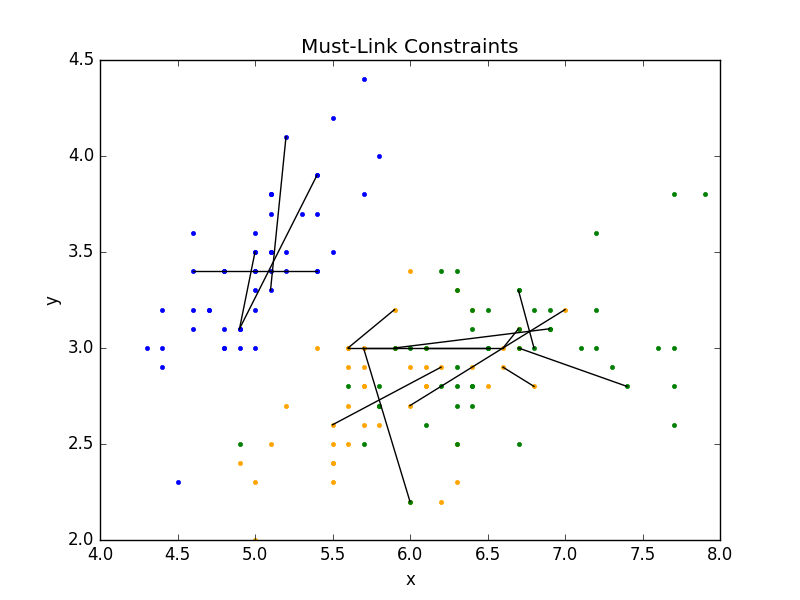
\includegraphics[width=.5\linewidth]{imagenes/c6/Restr/IrisML}}
	\subfloat[Restricciones \acs{CL}]
	{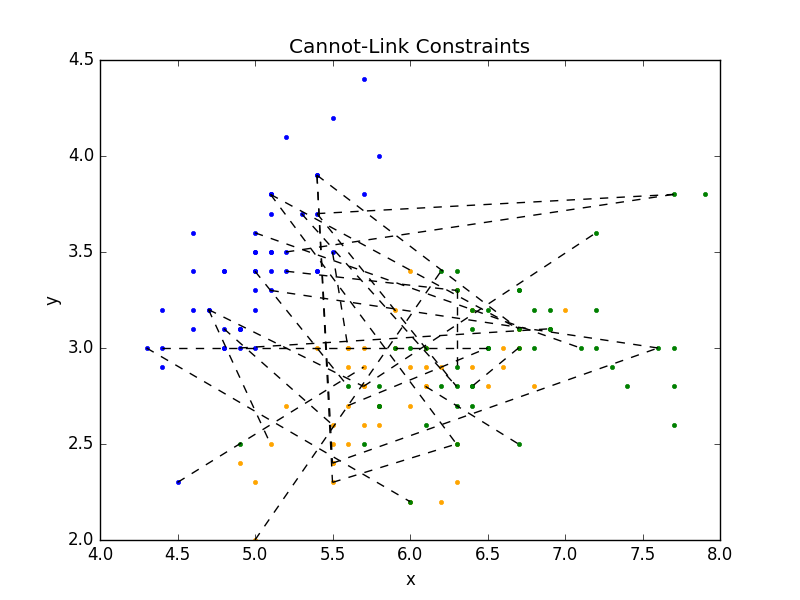
\includegraphics[width=.5\linewidth]{imagenes/c6/Restr/IrisCL}}\\
	\subfloat[Restricciones \acs{ML}]
	{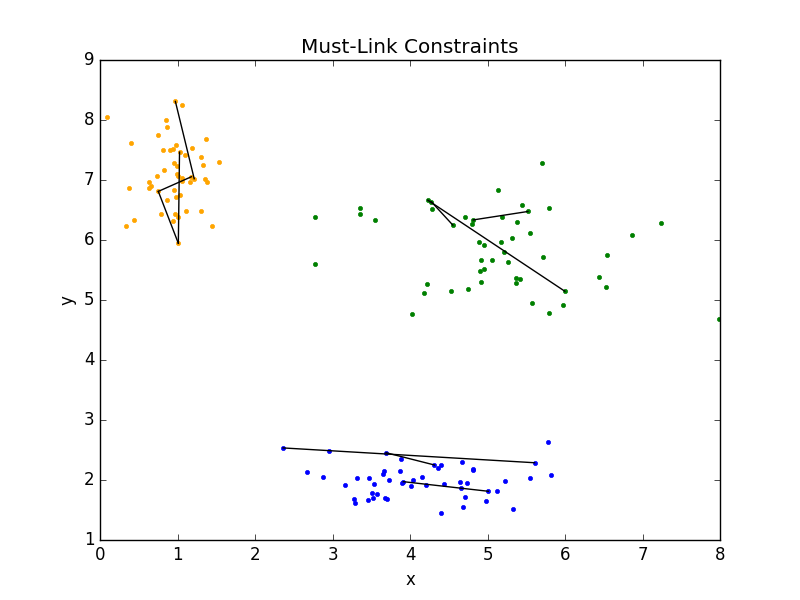
\includegraphics[width=.5\linewidth]{imagenes/c6/Restr/RandML}}
	\subfloat[Restricciones \acs{CL}]
	{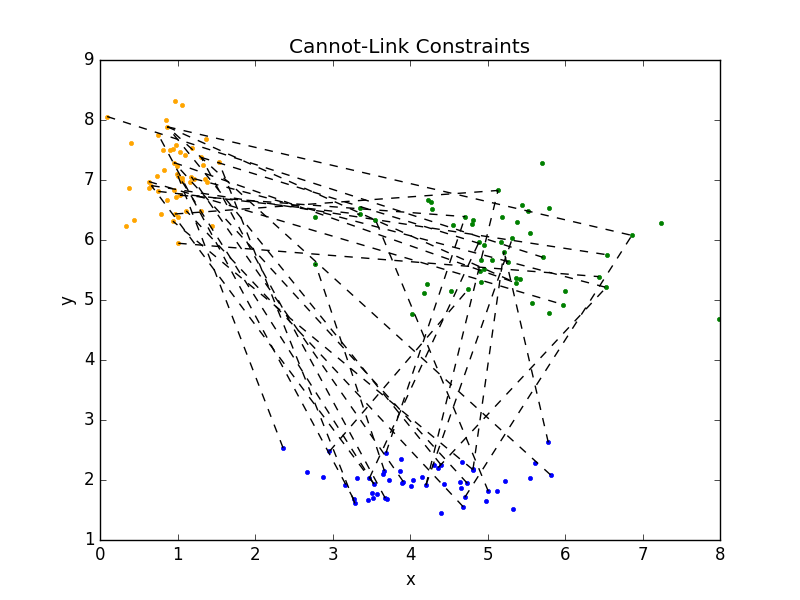
\includegraphics[width=.5\linewidth]{imagenes/c6/Restr/RandCL}}\\
	\caption{Visualización de las restricciones.}\label{fig:figure23}
\end{figure} 

\section{Resultados obtenidos con COP-K-Medias}

La Tabla \ref{tab:tabla5} muestra los resultados obtenidos al aplicar el algoritmo COP-K-Medias (Sección \ref{copkm}) a los conjuntos de datos presentados en la Sección \ref{datasets}. En ella se indican: el valor para \textit{Rand Index}, el tiempo que tarda el algoritmo en proporcionar salida, y el porcentaje de restricciones \acs{ML} y \acs{CL}. El número de restricciones generado para cada conjunto de datos es un $10\%$ del total de datos disponibles en cada caso, por tanto la suma del porcentaje de restricciones de los dos tipos debe ser aproximadamente $0.1$.

\begin{table}[!h]
	\centering
	\setlength{\arrayrulewidth}{1mm}
	\setlength{\tabcolsep}{10pt}
	\renewcommand{\arraystretch}{0.75}
	
	\rowcolors{2}{gray!25}{white}
	\begin{tabular}{ >{\centering\arraybackslash}m{2.5cm}  >{\centering\arraybackslash}m{1.8cm}>{\centering\arraybackslash}m{1.5cm}>{\centering\arraybackslash}m{1.2cm}>{\centering\arraybackslash}m{1.2cm}}
		\hline
		\rowcolor{black}
		\multicolumn{5}{c}{\bf \color{white}{Resultados de COP-K-Medias con restricciones CL y ML}}\\
		\hline
		\rowcolor{gray!50}
		\textbf{Dataset} & \textbf{RandIndex} & \textbf{Tiempo} & \textbf{\% ML} & \textbf{\% CL}  \\
		Iris & $0.499$ & $0.0532$ & $0.033$ & $0.066$ \\
		Wine & $0.38$ & $0.087$ & $0.056$ & $0.039$ \\
		Glass  & $0.25$ & $0.1449$ & $0.15$ & $0.04$ \\
		Breast Cancer & NA & NA & $0.028$ & $0.07$ \\ 
		Digits & $0.632$ & $13.306$ & $0.008$ & $0.092$ \\
		Rand & $0.960$ & $0.0346$ & $0.033$ & $0.066$ \\
		Spirals & $0.0245$ & $0.13$ & $0.05$ & $0.05$ \\
		Circles & $-0.002$ & $0.16$ & $0.046$ & $0.053$ \\
		Moons & NA & NA & $0.053$ & $0.046$ \\
		\hline
		
	\end{tabular}
	\caption{Resultados obtenidos con COP-K-Medias empleando restricciones \acs{CL} y \acs{ML}.}
	\label{tab:tabla5}
\end{table}

De entre los resultados obtenidos destacan los asociados a los conjuntos de datos \textit{Glass Dataset} y \textit{Moons Dataset}. Encontramos que en ninguno de los dos casos el algoritmo COP-K-Medias es capaz de encontrar una solución factible, a pesar de que es seguro que ésta existe, ya que las restricciones se generan en base a las etiquetas verdaderas. Esto es consecuencia directa de lo expuesto en la Observación \ref{ob:observacion34}, puesto que en la resolución del problema se emplean tanto restricciones de tipo \acs{ML} como \acs{CL}. Para obtener resultados para \textit{Glass Dataset} y \textit{Moons Dataset} podemos aplicar transformaciones a las restricciones para hacer el problema más simple (tratable), esto es, suprimir las restricciones de tipo \acs{CL} y aumentar las de tipo \acs{ML}, tal y como especificamos en la Sección \ref{Problemas}. La Tabla \ref{tab:tabla6} muestra los resultados con esta nueva configuración.

\begin{table}[!h]
	\centering
	\setlength{\arrayrulewidth}{1mm}
	\setlength{\tabcolsep}{10pt}
	\renewcommand{\arraystretch}{0.75}
	
	\rowcolors{2}{gray!25}{white}
	\begin{tabular}{ >{\centering\arraybackslash}m{2.5cm}  >{\centering\arraybackslash}m{1.8cm}>{\centering\arraybackslash}m{1.5cm}>{\centering\arraybackslash}m{1.2cm}>{\centering\arraybackslash}m{1.2cm}}
		\hline
		\rowcolor{black}
		\multicolumn{5}{c}{\bf \color{white}{Resultados de COP-K-Medias con restricciones ML}}\\
		\hline
		\rowcolor{gray!50}
		\textbf{Dataset} & \textbf{RandIndex} & \textbf{Tiempo} & \textbf{\% ML} & \textbf{\% CL}  \\
		Iris & $0.489$ & $0.0423$ & $0.366$ & $0$ \\
		Wine & $0.337$ & $0.0762$ & $0.353$ & $0$ \\
		Glass & $0.175$ & $0.112$ & $0.555$ & $0$ \\
		Breast Cancer & $0.45$ & $0.556$ & $0.224$ & $0$ \\
		Digits & $0.582$ & $10.847$ & $0.105$ & $0$ \\
		Rand & $1.0$ & $0.031$ & $0.393$ & $0$ \\
		Spirals & $-0.0028$ & $0.1302$ & $0.52$ & $0$ \\
		Circles & $0.091$ & $0.1301$ & $0.463$ & $0$ \\
		Moons & $0.126$ & $0.116$ & $0.513$ & $0$ \\
		\hline
		
	\end{tabular}
	\caption{Resultados obtenidos con COP-K-Medias empleando sólo restricciones \acs{ML}.}
	\label{tab:tabla6}
\end{table}

Como cabía esperar, los nuevos resultados muestran que, empleando sólo restricciones de tipo \acs{ML}, el algoritmo COP-K-Medias es capaz de dar una partición para todos los conjuntos de datos. Sin embargo, la precisión de las predicciones decrece en algunos casos; esto se debe la pérdida de la información que proporcionaban las restricciones \acs{CL}. 

Además de obtener los resultados numéricos, podemos representar algunas de las particiones obtenidas con COP-K-Medias para obtener una mejor idea del comportamiento del algoritmo. 

En la Figura \ref{fig:figure24} se muestran los resultados obtenidos para \textit{Iris Dataset} y \textit{Rand Dataset}; los cuadros (a) y (b) muestran los resultados considerando restricciones ML y CL, mientras que los (c) y (d) sólo consideran restricciones ML.

\begin{figure}[bth]
	\myfloatalign
	\subfloat[]
	{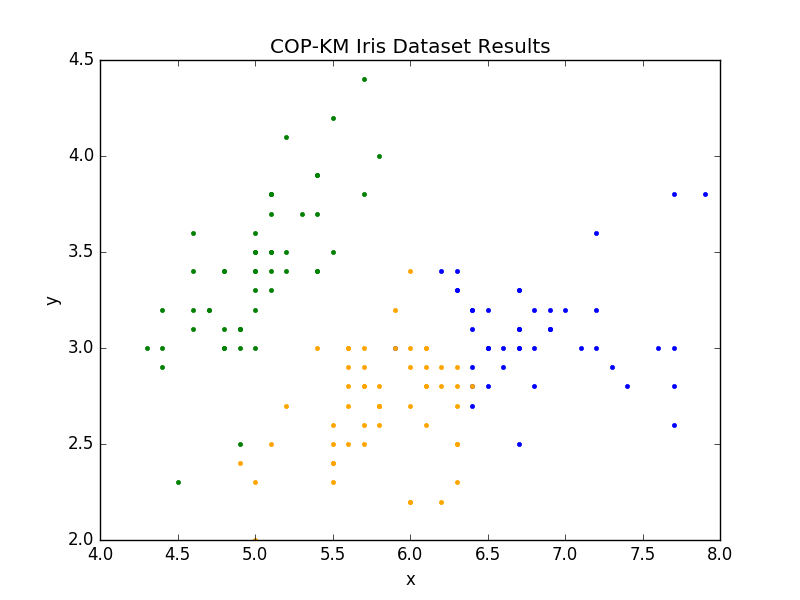
\includegraphics[width=.4\linewidth]{imagenes/c6/COPKM/Iris01}}
	\subfloat[]
	{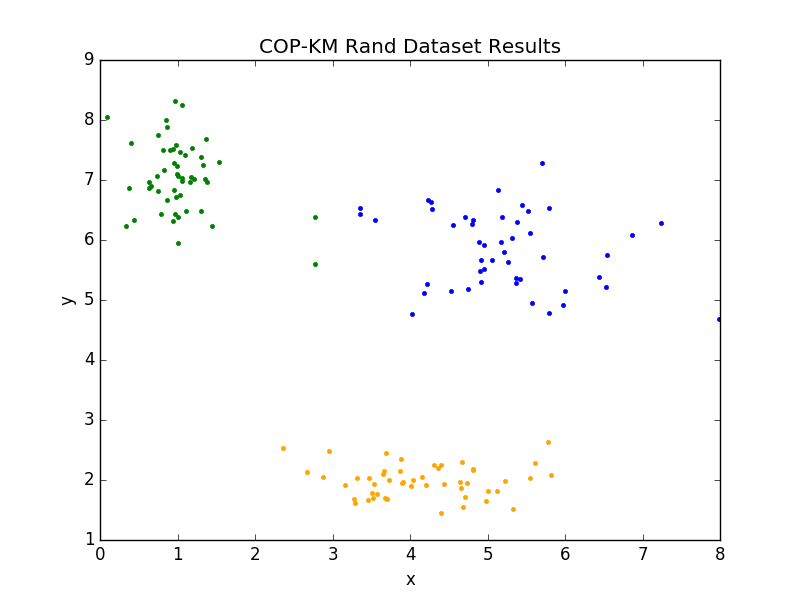
\includegraphics[width=.4\linewidth]{imagenes/c6/COPKM/Rand01}}\\
	\subfloat[]
	{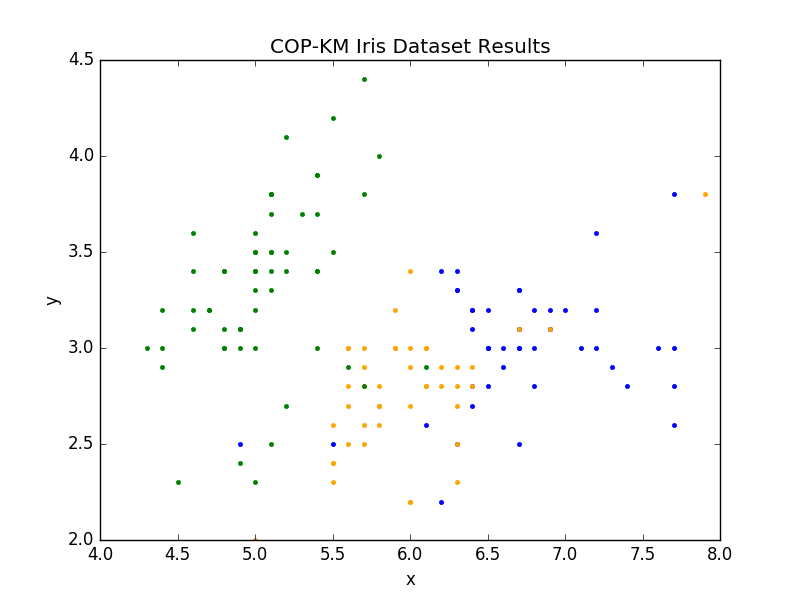
\includegraphics[width=.4\linewidth]{imagenes/c6/COPKM/IrisSoloML}}
	\subfloat[]
	{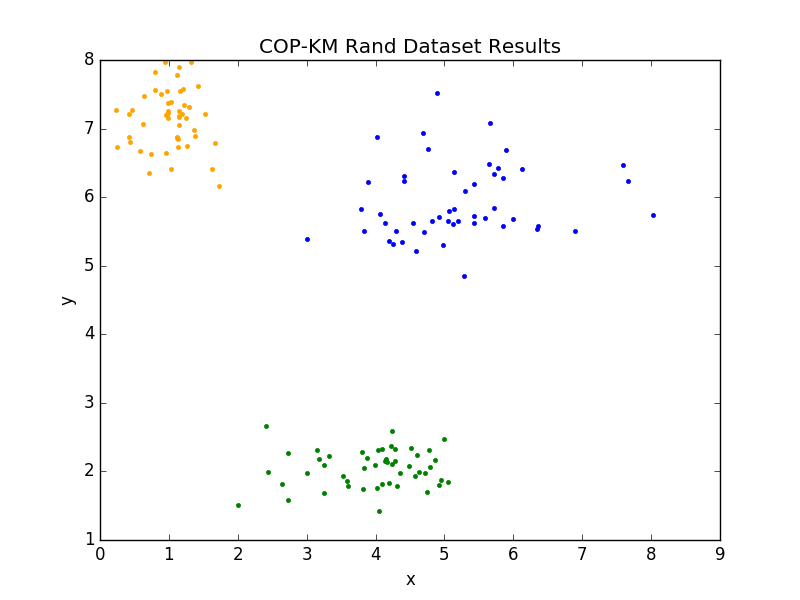
\includegraphics[width=.4\linewidth]{imagenes/c6/COPKM/RandSoloMl}}\\
	\caption{Visualización de los resultados de COP-K-Medias.}\label{fig:figure24}
\end{figure}

En la Figura \ref{fig:figure24} destacan las instancias del conjunto de datos \textit{Iris Dataset} que parecen estar dentro de un cluster distinto al que pertenecen. Es en estos casos en los que destaca la influencia de las restricciones en el proceso de asignación de instancias a clusters, ya que el algoritmo K-Medias (Apéndice \ref{ap:kmeans}) nunca proporcionaría esta partición como resultado.

\clearpage

\section{Resultados obtenidos con CEKM}

La Tabla \ref{tab:tabla8} muestra los resultados obtenidos al aplicar el algoritmo \acf{CEKM} (Sección \ref{cekm}) a los conjuntos de datos presentados en la Sección \ref{datasets}. Emplearemos un número de restricciones igual al $25\%$ del total de ejemplos disponibles para cada conjunto de datos. \footnote{Para obtener resultados con \acs{CEKM} para \textit{Breast Cancer Dataset} es necesario modificar el parámetro \texttt{stop\_thr}, y establecerlo a $0.1$ }

\begin{table}[!h]
	\centering
	\setlength{\arrayrulewidth}{1mm}
	\setlength{\tabcolsep}{10pt}
	\renewcommand{\arraystretch}{0.9}
	
	\rowcolors{2}{gray!25}{white}
	\begin{tabular}{ >{\centering\arraybackslash}m{2.5cm}  >{\centering\arraybackslash}m{1.8cm}>{\centering\arraybackslash}m{1.5cm}}
		\hline
		\rowcolor{black}
		\multicolumn{3}{c}{\bf \color{white}{Resultados obtenidos con CEKM}}\\
		\hline
		\rowcolor{gray!50}
		\textbf{Dataset} & \textbf{RandIndex} & \textbf{Tiempo}  \\
		Iris & $0.554$ & $9.567$  \\
		Wine & $0.395$ & $14.48$  \\
		Glass & NA & NA  \\
		Breast Cancer & $0.491$ & $64.22$  \\
		Digits & NA & NA  \\
		Rand & $0.950$ & $9.411$  \\
		Spirals & $0.061$ & $9.839$  \\
		Circles & $-0.0030$ & $12.588$  \\
		Moons & $0.247$ & $11.191$  \\
		\hline
		
	\end{tabular}
	\caption{Resultados obtenidos con \acs{CEKM}.}
	\label{tab:tabla8}
\end{table}

En ella destacan los resultados obtenidos para los conjuntos de datos \textit{Glass Dataset} y \textit{Digits Dataset}. El algoritmo \acs{CEKM} no es capaz de dar resultado para estos dos conjuntos de datos, debido a que las estructuras de memoria que lo soportan crecen de manera exponencial con $K$. La figura \ref{fig:figure25} muestra los resultados obtenidos con \acs{CEKM} para los conjuntos de datos \textit{Iris Dataset} y \textit{Rand Dataset}.

\begin{figure}[bth]
	\myfloatalign
	\subfloat[Resultados para \textit{Iris Dataset}]
	{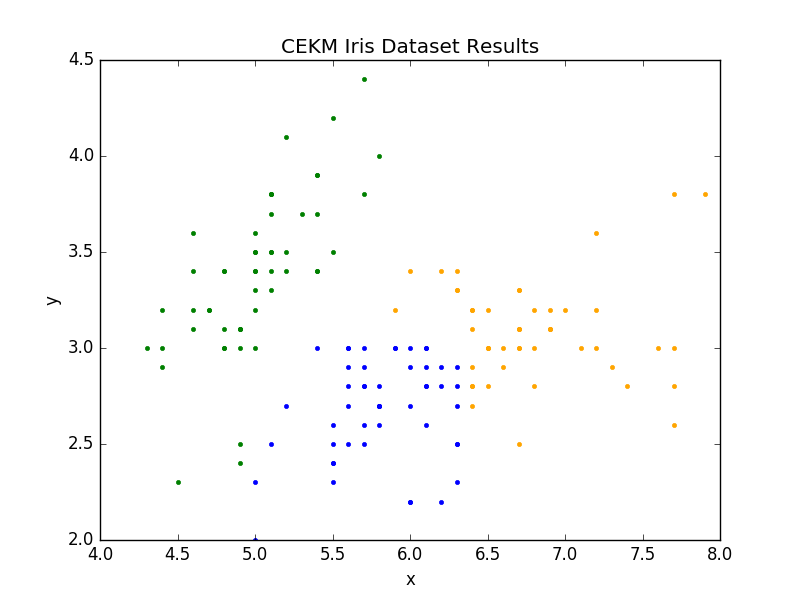
\includegraphics[width=.5\linewidth]{imagenes/c6/CEKM/CEKMIrisResult}}
	\subfloat[Resultados para \textit{Rand Dataset}]
	{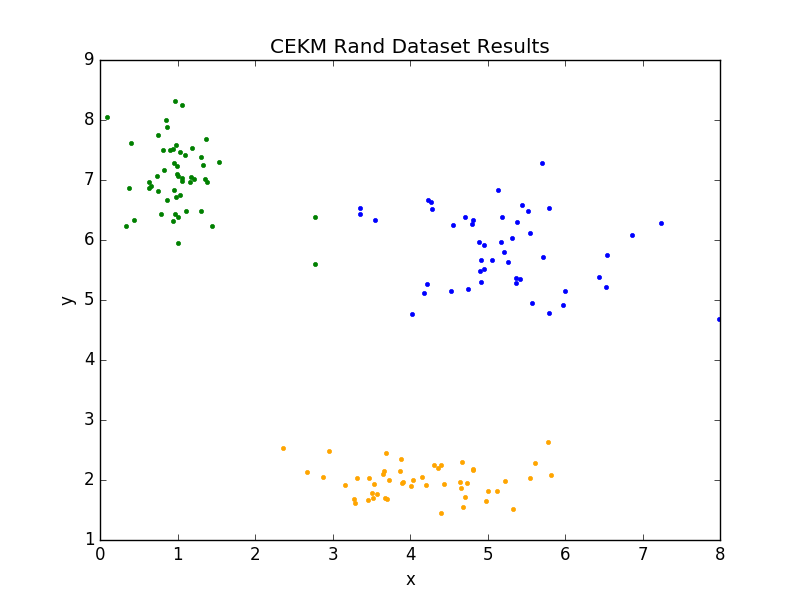
\includegraphics[width=.5\linewidth]{imagenes/c6/CEKM/CEKMRandResult}}
	\caption{Visualización de los resultados de \acs{CEKM}.}\label{fig:figure25}
\end{figure}

\clearpage

\section{Resultados obtenidos con LCVQE}

La Tabla \ref{tab:tabla8} muestra los resultados obtenidos al aplicar el algoritmo \acf{LCVQE} (Sección \ref{lcvqe}) a los conjuntos de datos presentados en la Sección \ref{datasets}. Daremos como parámetro para los centroides iniciales los calculados con el algoritmo K-Medias (Apéndice \ref{ap:kmeans}). Respecto al número de restricciones empleadas, será un $25\%$ del total de ejemplos disponibles para cada conjunto de datos.

\begin{table}[!h]
	\centering
	\setlength{\arrayrulewidth}{1mm}
	\setlength{\tabcolsep}{10pt}
	\renewcommand{\arraystretch}{0.9}
	
	\rowcolors{2}{gray!25}{white}
	\begin{tabular}{ >{\centering\arraybackslash}m{2.5cm}  >{\centering\arraybackslash}m{1.8cm}>{\centering\arraybackslash}m{1.5cm}}
		\hline
		\rowcolor{black}
		\multicolumn{3}{c}{\bf \color{white}{Resultados obtenidos con LCVQE}}\\
		\hline
		\rowcolor{gray!50}
		\textbf{Dataset} & \textbf{RandIndex} & \textbf{Tiempo}  \\
		Iris & $0.663$ & $0.141$  \\
		Wine & $0.390$ & $0.002$  \\
		Glass & $0.197$ & $0.002$  \\
		Breast Cancer & $0.616$ & $0.003$  \\
		Digits & $0.680$ & $0.062$  \\
		Rand & $0.989$ & $0.001$  \\
		Spirals & $0.057$ & $0.002$  \\
		Circles & $-0.003$ & $0.005$  \\
		Moons & $0.215$ & $0.002$  \\
		\hline
		
	\end{tabular}
	\caption{Resultados obtenidos con \acs{LCVQE}.}
	\label{tab:tabla9}
\end{table}

De nuevo, podemos obtener una representación de algunos de los mejores resultados obtenidos con \acs{LCVQE}. La figura \ref{fig:figure26} muestra los resultados obtenidos con \acs{LCVQE} para los conjuntos de datos \textit{Iris Dataset} y \textit{Rand Dataset}. 


\begin{figure}[bth]
	\myfloatalign
	\subfloat[Resultados para \textit{Iris Dataset}]
	{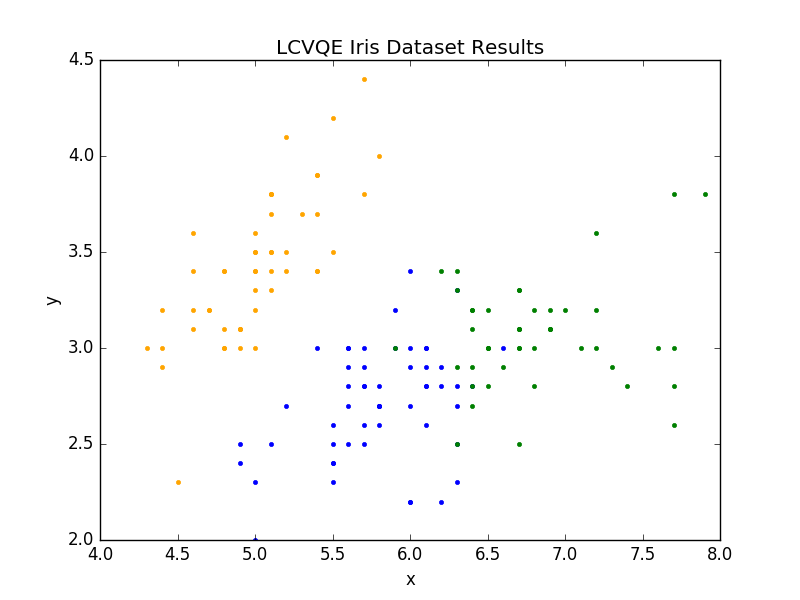
\includegraphics[width=.5\linewidth]{imagenes/c6/LCVQE/LCVQEIris}}
	\subfloat[Resultados para \textit{Rand Dataset}]
	{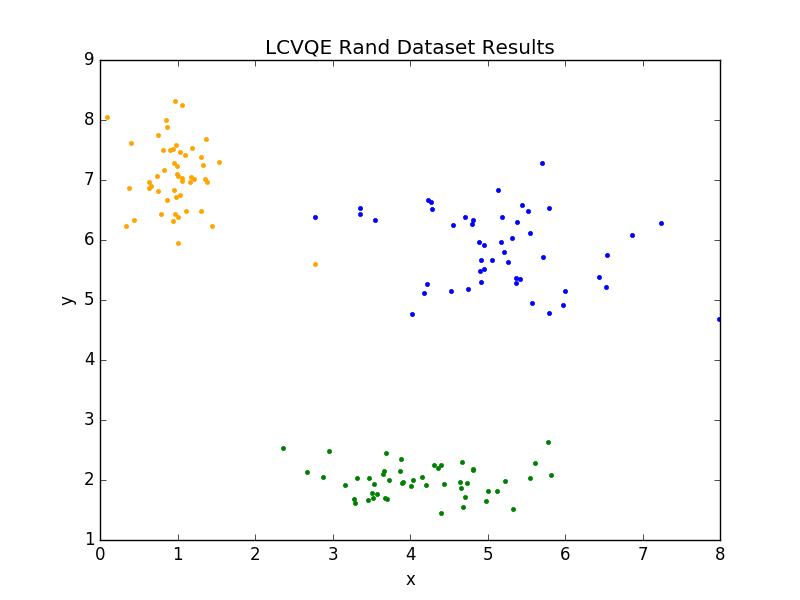
\includegraphics[width=.5\linewidth]{imagenes/c6/LCVQE/LCVQERand}}
	\caption{Visualización de los resultados de \acs{LCVQE}.}\label{fig:figure26}
\end{figure}

\clearpage

\section{Resultados obtenidos con RDP-Means}

La Tabla \ref{tab:tabla10} muestra los resultados obtenidos al aplicar el algoritmo \acf{RDPM} (Sección \ref{rdpmYtvc}) a los conjuntos de datos presentados en la Sección \ref{datasets}. Para aplicar \acs{RDPM} es necesario especificar el parámetro $\lambda$; en este caso este parámetro se calcula de manera experimental y en base a las distancia medias entre instancias dentro del conjunto de datos. De igual forma que en el caso anterior, especificaremos el número de restricciones como un $25\%$ del total de ejemplos disponibles para cada conjunto de datos.

\begin{table}[!h]
	\centering
	\setlength{\arrayrulewidth}{1mm}
	\setlength{\tabcolsep}{10pt}
	\renewcommand{\arraystretch}{0.85}
	
	\rowcolors{2}{gray!25}{white}
	\begin{tabular}{ >{\centering\arraybackslash}m{2.5cm}  >{\centering\arraybackslash}m{1.8cm}>{\centering\arraybackslash}m{1.5cm}>{\centering\arraybackslash}m{1cm}>{\centering\arraybackslash}m{1cm}}
		\hline
		\rowcolor{black}
		\multicolumn{5}{c}{\bf \color{white}{Resultados obtenidos con RDPM}}\\
		\hline
		\rowcolor{gray!50}
		\textbf{Dataset} & \textbf{RandIndex} & \textbf{Tiempo} & \textbf{$\lambda$} & \textbf{$K_{out}$}  \\
		Iris & $0.479$ & $0.508$ & $1.7$ & $3$ \\
		Wine & $0.342$ & $0.598$ & $438.11$ & $3$ \\
		Glass & $0.255$ & $0.785$ & $2.214$ & $6$ \\
		Breast Cancer & $0.501$ & $14.096$ & $2833.35$ & $3$ \\
		Digits & $0.665$ & $177.12$ & $44.14$ & $17$ \\
		Rand & $0.98$ & $0.365$ & $4$ & $3$ \\
		Spirals & $0.0147$ & $2.683$ & $13.83$ & $3$ \\
		Circles & $-0.003$ & $1.27$ & $1.5$ & $2$  \\
		Moons & $0.234$ & $1.563$ & $2$ & $2$ \\
		\hline
		
	\end{tabular}
	\caption{Resultados obtenidos con \acs{RDPM}.}
	\label{tab:tabla10}
\end{table}

En la Tabla \ref{tab:tabla10} la columna $K_{out}$ representa el número de clases de la partición de salida proporcionada por \acs{LCVQE}. Podemos estudiar la influencia del parámetro $\lambda$ sobre este resultado. Para ello, ejecutamos el algoritmo especificando en cada caso un $\lambda$ mayor. La Tabla \ref{tab:tabla11} muestra los resultados obtenidos con esta nueva configuración.

\begin{table}[!h]
	\centering
	\setlength{\arrayrulewidth}{1mm}
	\setlength{\tabcolsep}{10pt}
	\renewcommand{\arraystretch}{0.85}
	
	\rowcolors{2}{gray!25}{white}
	\begin{tabular}{ >{\centering\arraybackslash}m{2.5cm}  >{\centering\arraybackslash}m{1.8cm}>{\centering\arraybackslash}m{1.5cm}>{\centering\arraybackslash}m{1cm}>{\centering\arraybackslash}m{1cm}}
		\hline
		\rowcolor{black}
		\multicolumn{5}{c}{\bf \color{white}{Resultados obtenidos con RDPM para un mayor $\lambda$}}\\
		\hline
		\rowcolor{gray!50}
		\textbf{Dataset} & \textbf{RandIndex} & \textbf{Tiempo} & \textbf{$\lambda_{mayor}$} & \textbf{$K_{out}$}  \\
		Iris & $0.321$ & $0.683$ & $2$ & $2$ \\
		Wine & $0.313$ & $0.691$ & $538.11$ & $3$ \\
		Glass & $0$ & $0.505$ & $4.214$ & $3$ \\
		Breast Cancer & $0.491$ & $11.236$ & $3833.35$ & $2$ \\
		Digits & $0.268$ & $144.96$ & $60.14$ & $4$ \\
		Rand & $0$ & $0.26$ & $7$ & $1$ \\
		Spirals & $0$ & $0.969$ & $20.5$ & $1$ \\
		Circles & $0$ & $0.965$ & $4.5$ & $1$  \\
		Moons & $0$ & $0.97$ & $5$ & $1$ \\
		\hline
		
	\end{tabular}
	\caption{Resultados obtenidos con \acs{RDPM} especificando un mayor $\lambda$.}
	\label{tab:tabla11}
\end{table}

A la vista de los resultados expuestos en la Tabla \ref{tab:tabla11} podemos decir que escoger $\lambda$ es equivalente a escoger $K$ en los algoritmos que toman como parámetro el número de clusters de la partición de salida. Por tanto, es crucial realizar un estudio sobre este parámetro para resolver el problema concreto al que nos enfrentemos. En la Figura \ref{fig:figure28} representamos los resultados obtenidos con las diferentes elecciones de $\lambda$ para los conjuntos de datos \textit{Iris Dataset} y \textit{Rand Dataset}. 

\begin{figure}[bth]
	\myfloatalign
	\subfloat[ \textit{Iris Dataset} con $\lambda = 1.7$]
	{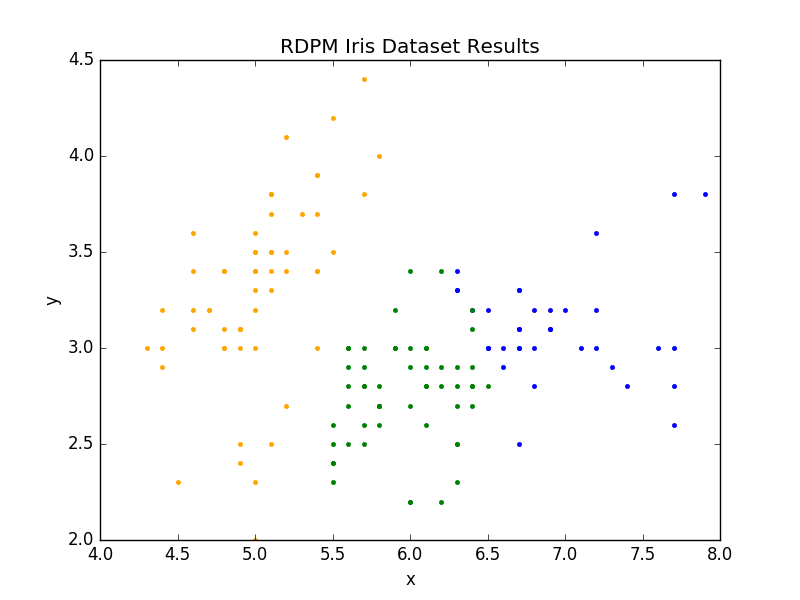
\includegraphics[width=.5\linewidth]{imagenes/c6/RDPM/RDPMIris1}}
	\subfloat[ \textit{Iris Dataset} con $\lambda = 2$]
	{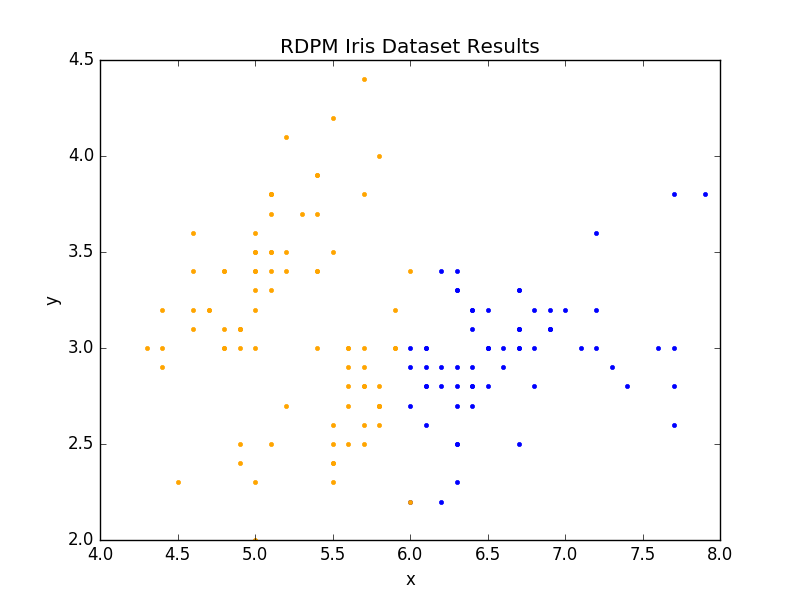
\includegraphics[width=.5\linewidth]{imagenes/c6/RDPM/RDPMIris2}}\\
	\subfloat[ \textit{Rand Dataset} con $\lambda = 4$]
	{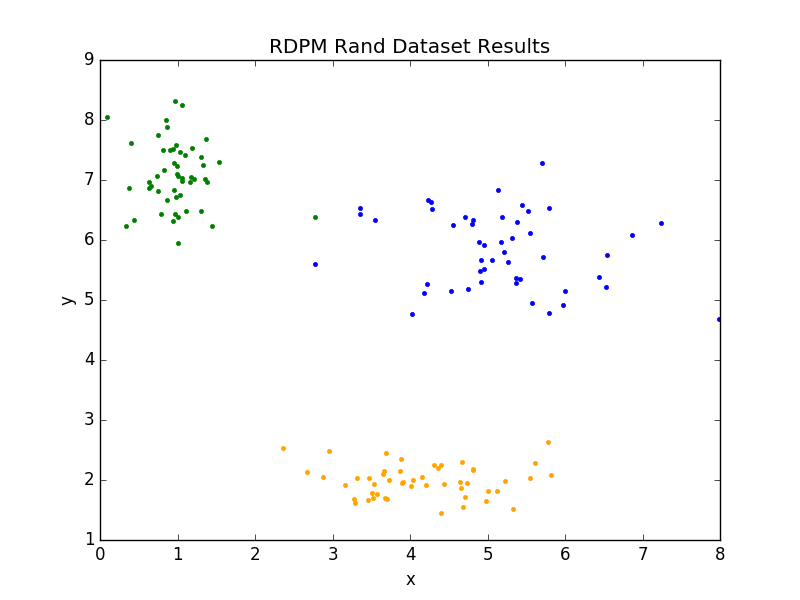
\includegraphics[width=.5\linewidth]{imagenes/c6/RDPM/RDPMRand1}}
	\subfloat[ \textit{Rand Dataset} con $\lambda = 7$]
	{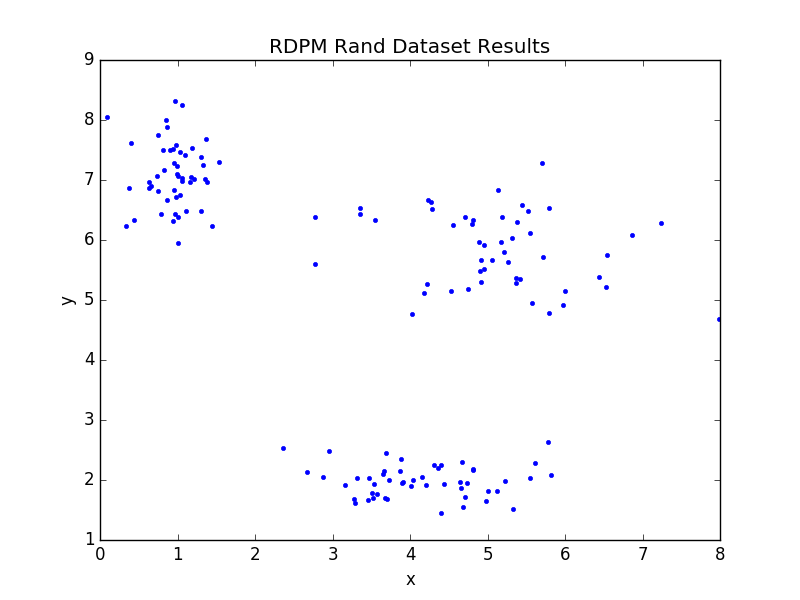
\includegraphics[width=.5\linewidth]{imagenes/c6/RDPM/RDPMRand2}}\\
	\caption{Visualización de los resultados de RDPM con diferentes valores de $\lambda$.}\label{fig:figure28}
\end{figure}

La Figura \ref{fig:figure28} refleja claramente la influencia del parámetro $\lambda$ en la partición que \acs{RDPM} proporciona como resultado del proceso de clustering que lleva a cabo. En el caso del conjunto de datos \textit{Iris Dataset}, bastan 3 décimas de diferencia en $\lambda$ para que el resultado degenere en una partición de dos clusters en lugar de 3.

\clearpage

\section{Resultados obtenidos con TVClust}

La Tabla \ref{tab:tabla11} muestra los resultados obtenidos al aplicar el algoritmo \acf{TVClust} (Sección \ref{rdpmYtvc}) a los conjuntos de datos presentados en la Sección \ref{datasets}. Especificamos el número de restricciones como un $25\%$ del total de ejemplos disponibles para cada conjunto de datos, tal y como hicimos en los casos anteriores.

\begin{table}[!h]
	\centering
	\setlength{\arrayrulewidth}{1mm}
	\setlength{\tabcolsep}{10pt}
	\renewcommand{\arraystretch}{0.9}
	
	\rowcolors{2}{gray!25}{white}
	\begin{tabular}{ >{\centering\arraybackslash}m{2.5cm}  >{\centering\arraybackslash}m{1.8cm}>{\centering\arraybackslash}m{1.5cm}}
		\hline
		\rowcolor{black}
		\multicolumn{3}{c}{\bf \color{white}{Resultados obtenidos con TVClust}}\\
		\hline
		\rowcolor{gray!50}
		\textbf{Dataset} & \textbf{RandIndex} & \textbf{Tiempo}  \\
		Iris & $0.532$ & $0.342$  \\
		Wine & $0.176$ & $0.5$  \\
		Glass & $0.26$ & $3.332$  \\
		Breast Cancer & $0$ & $1.3$  \\
		Digits & $0.680$ & $78.46$  \\
		Rand & $0.941$ & $0.83$  \\
		Spirals & $0.042$ & $0.3$  \\
		Circles & $0.075$ & $1.7$  \\
		Moons & $0.576$ & $5.59$  \\
		\hline
		
	\end{tabular}
	\caption{Resultados obtenidos con \acs{TVClust}.}
	\label{tab:tabla12}
\end{table}

Destaca el resultado obtenido para el conjunto de datos \textit{Breast Cancer Dataset}, para el que \acs{TVClust} no es capaz de encontrar una partición mínimamente acertada. Esto puede deberse a la alta dimensionalidad del conjunto de datos. La Figura \ref{fig:figure28} muestra los resultados obtenidos con \acs{TVClust} para los conjuntos de datos \textit{Iris Dataset} y \textit{Rand Dataset}. 


\begin{figure}[bth]
	\myfloatalign
	\subfloat[Resultados para \textit{Iris Dataset}]
	{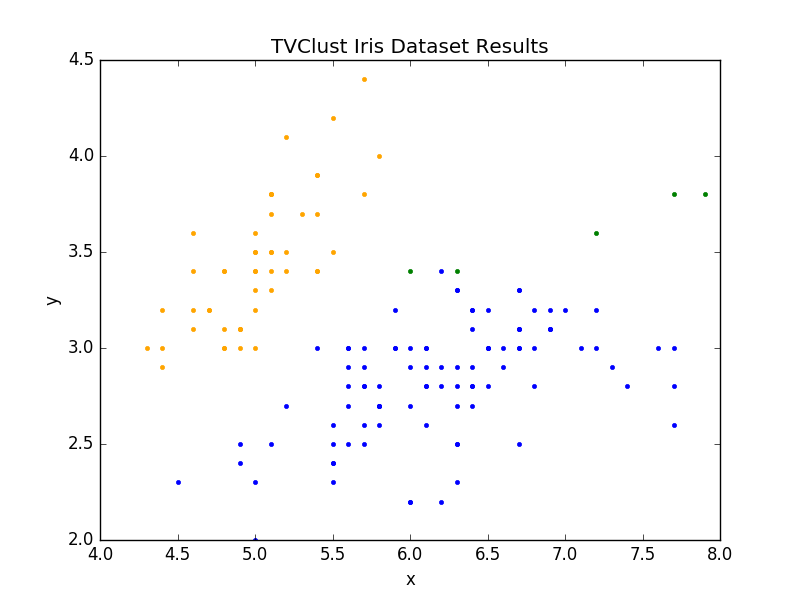
\includegraphics[width=.5\linewidth]{imagenes/c6/TVClust/TVIris}}
	\subfloat[Resultados para \textit{Rand Dataset}]
	{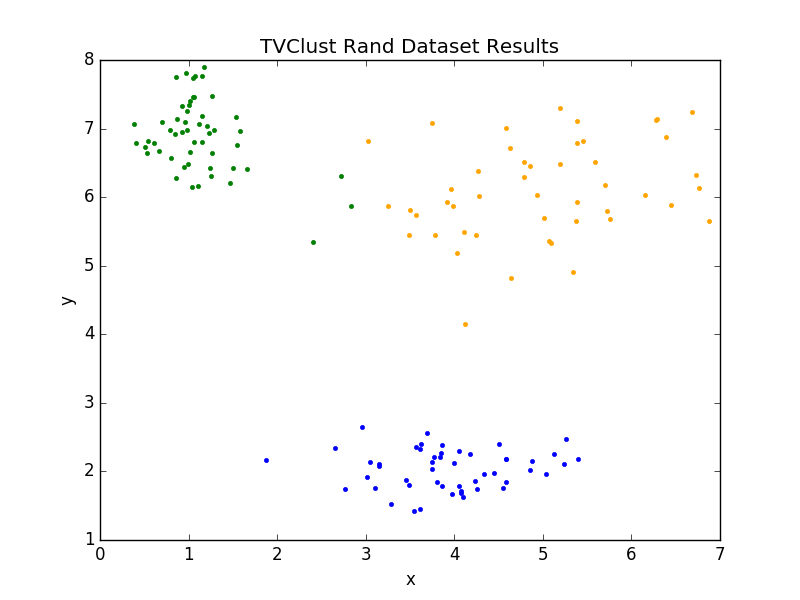
\includegraphics[width=.5\linewidth]{imagenes/c6/TVClust/TVRand}}
	\caption{Visualización de los resultados de \acs{TVClust}.}\label{fig:figure29}
\end{figure}

\clearpage

\section{Comparativa general de resultados}

La Tabla \ref{tab:tabla13} muestra los resultados obtenidos por cada algoritmo para cada conjunto de datos, en lo que a precisión en las predicciones se refiere. Salvo algunas excepciones, todos los algoritmos se comportan de manera similar bajo las condiciones descritas al inicio del Capítulo \ref{ch:Experimentación}. Destaca la precisión en las predicciones sobre el conjunto de datos \textit{Rand Dataset}, así como la pobreza de las mismas sobre el conjunto \textit{Circles Dataset}.

\begin{table}[!h]
	\centering
	\setlength{\arrayrulewidth}{1mm}
	\setlength{\tabcolsep}{9pt}
	\renewcommand{\arraystretch}{0.8}
	
	\rowcolors{2}{gray!25}{white}
	\begin{tabular}{ >{\centering\arraybackslash}m{2.5cm}  >{\centering\arraybackslash}m{1.2cm}>{\centering\arraybackslash}m{1.1cm}>{\centering\arraybackslash}m{1.1cm}>{\centering\arraybackslash}m{1.1cm}>{\centering\arraybackslash}m{1.3cm}}
		\hline
		\rowcolor{black}
		\multicolumn{6}{c}{\bf \color{white}{Comparativa General de Resultados (RandIndex)}}\\
		\hline
		\rowcolor{gray!50}
		\textbf{Dataset} & \textbf{COPKM} & \textbf{CEKM} & \textbf{LCVQE} & \textbf{RDPM} & \textbf{TVClust}  \\
		Iris & $0.489$  & $0.554 $ & $\boldsymbol{0.663}$ & $0.479 $ & $0.532 $ \\
		Wine & $0.337$  & $\boldsymbol{0.395}$ & $0.390$ & $0.342 $ & $0.176 $ \\
		Glass & $0.175$  & NA & $0.197 $ & $\boldsymbol{0.255}$ & $0.26 $ \\
		Breast Cancer & $0.45$ & $0.491 $ & $\boldsymbol{0.616}$ & $0.501 $ & $0 $ \\
		Digits & $0.582$ & NA & $\boldsymbol{0.680}$ & $0.665 $ & $\boldsymbol{0.680}$ \\
		Rand & $\boldsymbol{1.0}$ & $0.950 $ & $0.989 $ & $0.98 $ & $0.941 $ \\
		Spirals & $-0.0028$ & $0.061 $ & $\boldsymbol{0.057}$  & $0.0147 $ & $0.042 $ \\
		Circles & $\boldsymbol{0.091}$  & $-0.003 $ & $-0.003 $ & $-0.003 $ & $0.075 $ \\
		Moons & $0.126$  & $0.247 $ & $0.215$ & $0.234 $ & $\boldsymbol{0.576}$ \\
		\hline
		
	\end{tabular}
	\caption{Comparativa general de resultados (RandIndex).}
	\label{tab:tabla13}
\end{table}

En lo que a tiempo de ejecución se refiere, la Tabla \ref{tab:tabla14} muestra las marcas obtenidas por cada algoritmo. Cabe destacar que, en los casos en los que un método toma menos de 1 segundo en proporcionar resultado, cualquier otro proceso ejecutando en la máquina puede perturbar las mediciones, por tanto no han de tomarse como medidas exactas, simplemente como indicadores generales.

\begin{table}[!h]
	\centering
	\setlength{\arrayrulewidth}{1mm}
	\setlength{\tabcolsep}{9pt}
	\renewcommand{\arraystretch}{0.8}
	
	\rowcolors{2}{gray!25}{white}
	\begin{tabular}{ >{\centering\arraybackslash}m{2.5cm}  >{\centering\arraybackslash}m{1.2cm}>{\centering\arraybackslash}m{1.1cm}>{\centering\arraybackslash}m{1.1cm}>{\centering\arraybackslash}m{1.1cm}>{\centering\arraybackslash}m{1.3cm}}
		\hline
		\rowcolor{black}
		\multicolumn{6}{c}{\bf \color{white}{Comparativa General de Resultados (Tiempo)}}\\
		\hline
		\rowcolor{gray!50}
		\textbf{Dataset} & \textbf{COPKM} & \textbf{CEKM} & \textbf{LCVQE} & \textbf{RDPM} & \textbf{TVClust}  \\
		Iris & $\boldsymbol{0.0423}$  & $9.567 $ & $0.141 $ & $0.508 $ & $0.683 $ \\
		Wine & $0.0762 $  & $14.48 $ & $\boldsymbol{0.002}$ & $0.598 $ & $0.691 $ \\
		Glass & $0.112 $  & NA & $\boldsymbol{0.002}$ & $0.785 $ & $0.505 $ \\
		Breast Cancer & $0.556 $ & $64.22 $ & $\boldsymbol{0.003}$ & $14.096 $ & $11.236 $\\
		Digits & $10.847 $ & NA & $\boldsymbol{0.062}$ & $177.12 $ & $144.96 $ \\
		Rand & $0.031 $ & $9.411 $ & $\boldsymbol{0.001}$ & $0.365 $ & $0.26 $ \\
		Spirals & $0.1302 $ & $9.839 $ & $\boldsymbol{0.002}$ & $2.683 $ & $0.969 $ \\
		Circles & $0.1301 $ & $12.588 $ & $\boldsymbol{0.005}$ & $1.27 $ & $0.965 $ \\
		Moons & $0.116 $ & $11.191 $ & $\boldsymbol{0.002}$ & $1.563 $ & $0.97 $ \\
		\hline
		
	\end{tabular}
	\caption{Comparativa general de resultados (Tiempo).}
	\label{tab:tabla14}
\end{table}

